\begin{appendices}
  \section{Hello}

  \begin{figure}
    
\includegraphics[width=14.0cm]{inc/output.pdf}
    \caption{Example Graph}
    \label{cap:adx:graph}
  \end{figure}

  \begin{figure}
    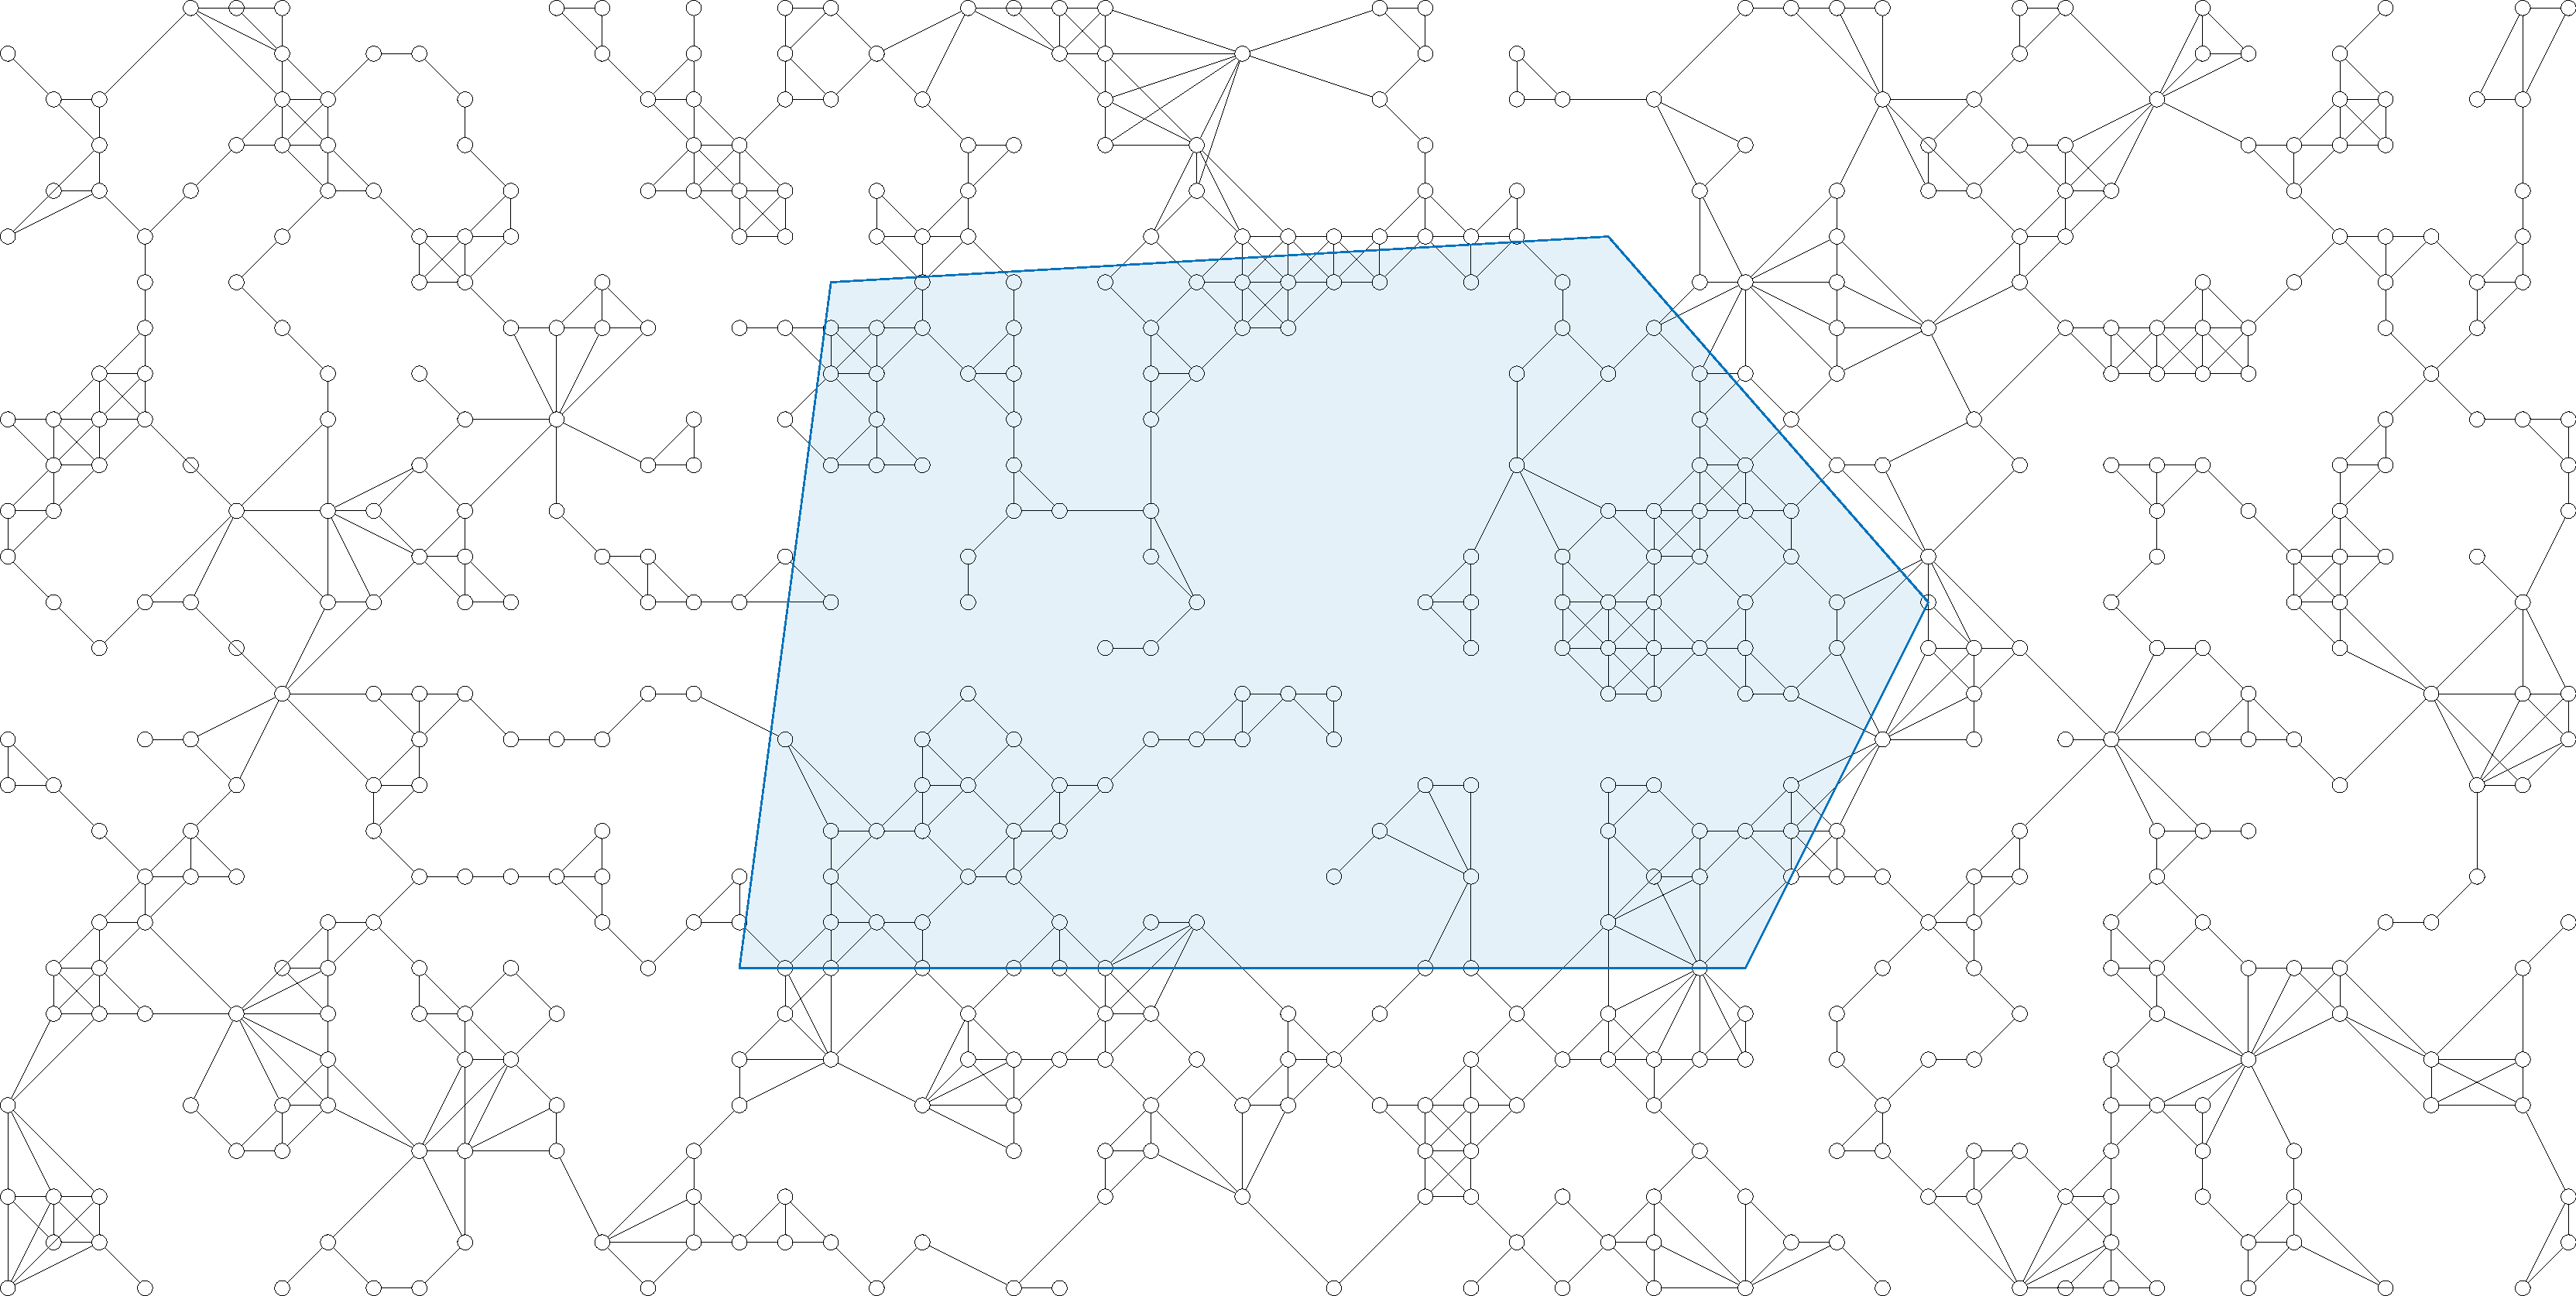
\includegraphics[width=14.0cm]{inc/output3.pdf}
    \caption{Example Graph}
    \label{cap:adx:graph}
  \end{figure}

  \begin{figure}
    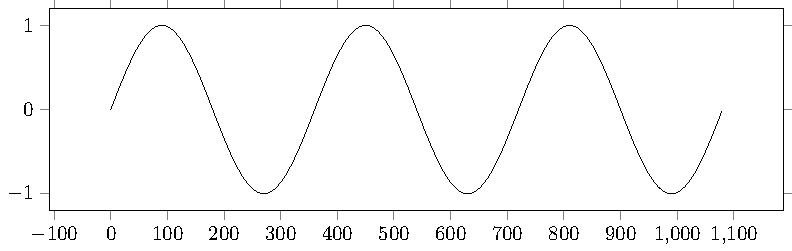
\includegraphics[width=14.0cm]{inc/plot.pdf}
    \caption{sin $f()$}
    \label{cap:adx:graph}
  \end{figure}

  \begin{table}[!htp]
    \caption{Please write a table caption here}
    \label{tab:A:1}
    \begin{tabular*}{14.0cm}{p{2.0cm}p{2.5cm}p{2.0cm}p{7.5cm}}
      \toprule
      Classes & Subclass & Length & Action Mechanism  \\
      \midrule
      Translation & mRNA$^a$  & 22 (19--25) & Translation repression, mRNA cleavage\\
      Translation & mRNA cleavage & 21 & mRNA cleavage\\
      Translation & mRNA  & 21--22 & mRNA cleavage\\
      Translation & mRNA  & 24--26 & Histone and DNA Modification\\
      \bottomrule
    \end{tabular*}
    $^a$ Table foot note (with superscript)
  \end{table}

    \subsection{This is important}
  \section{Graphs}
    \subsection{There is more to be said here}
\end{appendices}
